\chapter{Power Measurement}
\section{Trace collection}

Power traces need to be collected using a board called XBP. Figure~\ref{fig:xbp} shows how this device is connected to
the power supply and the DUT. The XBP includes a shunt resistor and an amplifier with selectable gain.
The XBP is connected to the digital oscilloscope using an SMA connector.
Power is supplied through the XBP to the DUT. The voltage drop across the shunt resistor is amplified and the oscilloscope records the amplified trace.
Figure~\ref{fig:power} shows an example trace collected using this setup. 


\begin{figure} 
   \begin{center}
   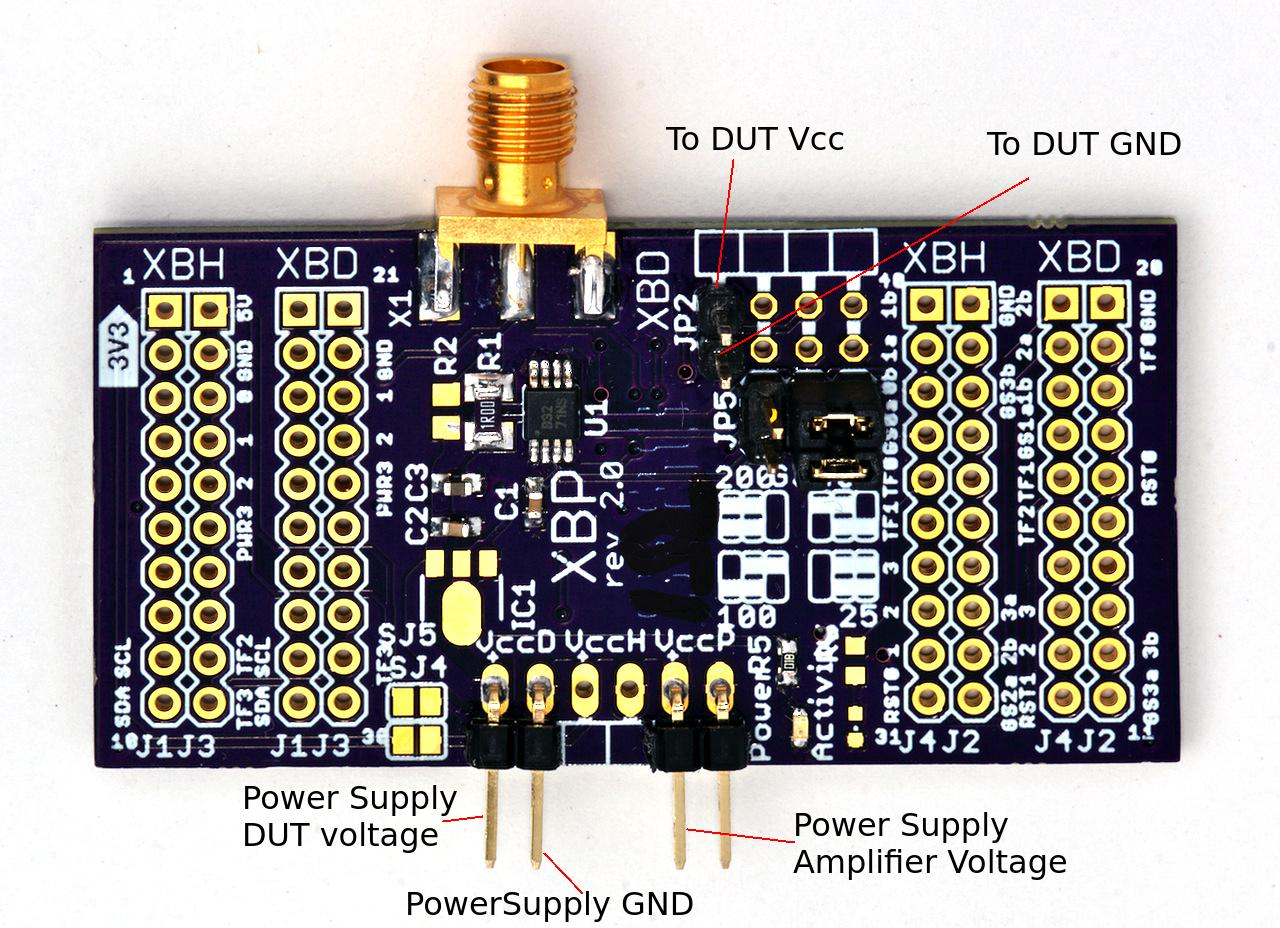
\includegraphics[scale=1]{../figures/xbp-no-xbh-labeled}
   \caption{\label{fig:xbp}The XBP Board}
   \end{center}
  
\end{figure}


\begin{figure} 
   \begin{center}
   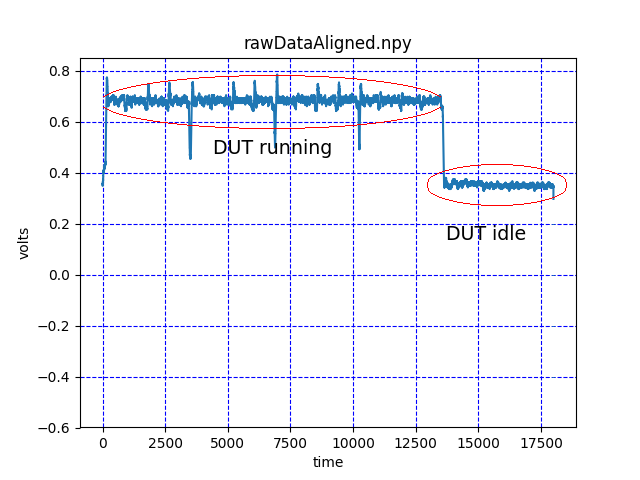
\includegraphics[scale=0.6]{../figures/power.png}
   \caption{\label{fig:power}The XBP Board}
   \end{center}
\end{figure}

\newline


\section{Power Measurement Configuration}
Before running the power measurement script, few configuration  parameters must be set. 
The configuration is located at \texttt{/fobos/config/analysis.ini}. Below is an example of the configuration and brief description
for the parameters.


\begin{verbatim}
[power]
#Source trace file (input)
srcFile         = rawDataAligned.npy
#File name to write the output
dstFile         = powerResults.txt
#Number of traces used in power calculation
numTraces       = 20
#sample number to start/end. Samples before and after
#will be ignored.
startSample     = 0
endSample       = 15000
\end{verbatim}

\section{Running the Power Measurement Script}

Run the \texttt{fobos/bin/calcPower.py} script.
This will display a menu showing all the measurements done in the current project.
You can select a measurement and the script will take it as input. A new analysis directory will be created under the selected project directory to store output files.
Power measurement will be displayed on the screen that shows minimum and average power. Below is a sample output file.

\begin{verbatim}
Source File: rawDataAligned.npy
Start sample (for truncated traces): 1
...
XBP Shunt Resistance (ohms): 1
...
Mean voltage for truncated traces is: 0.67885V
Mean power for truncated traces is: 0.0326W
\end{verbatim}
